\section{Ausgangssituation}
Zurzeit gibt es drei voneinander abhängige Programme, die die Aufnahme und Auswertung der Daten übernehmen. 
Die derzeit eingesetzten Programme können nur von einigen wenigen Fachkräften benutzt werden und sind unübersichtlich.

\section{Zielsetzung}
Zielsetzung ist eine Vereinfachung der Bedienung der Antriebsprüfstände. 
Des Weiteren eine Verbesserung der Datenauswertung mithilfe von Mustererkennung.
Außerdem eine Visualisierung der ausgewerteten Daten.
Abschließend soll auch die Fehlererkennung und -beseitigung erhöht werden.

\section{Funktionale Anforderungen}
\subsection{Analyse der vorhandenen Daten}  
\begin{figure}[h]
    \centering
    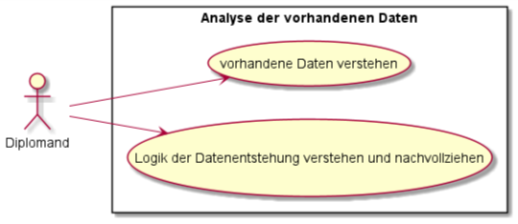
\includegraphics{pics/diplomand_anforderungen.png}
    \caption{Analyse der vorhandenen Daten}
    \label{fig:analyse}
\end{figure}

\begin{itemize}
    \item Der Diplomand soll die vorhandenen Daten analysieren, das beinhaltet welche Daten vorhanden sind, 
    wie groß die Datenmenge ist, ob die Daten auswertbar sind und was man in den Daten erkennt.
    \item Der Diplomand soll die Logik der Datenentstehung verstehen und nachvollziehen können, 
    das beinhaltet welche Signale vom System übermittelt werden, in welcher Qualität diese Signale kommen, 
    wie diese Signale in benutzbare Daten umgewandelt werden und wie die Schnittstelle aussieht und arbeitet.
\end{itemize}

\subsection{Antriebsprüfstands-Software zur Untersuchung und Qualitätssicherung von Zugteilen}
\begin{figure}[h]
    \centering
    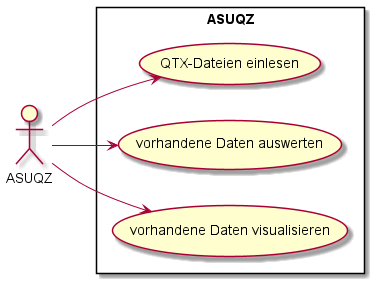
\includegraphics{pics/asuqz_anforderungen.png}
    \caption{ASUQZ Anforderungen}
    \label{fig:asuqz_anforderungen}
\end{figure}
\begin{itemize}
    \item Der Prototyp soll die vorhandenen QTX-Dateien, welche von dem derzeit benutzten Auswertungsprogramm der ÖBB produziert werden,
    einlesen können.
    \item Der Prototyp soll die vorhanden Daten nach Fehlern durchsuchen und ausgewerteten.
    \item Der Prototyp soll die ausgewerteten Daten graphisch darstellen.
\end{itemize}

\section{Nicht-funktionale Anforderungen}
\begin{itemize}
    \item Der Prototyp soll in Deutsch realisiert section
    \item Die Auswertung soll formatiert und leicht lesbar sein
    \item Der Prototyp soll in einer angemessenen Zeitspanne funktionieren und reagieren
    \item Die vorhandenen und im Laufe des Projekts erhobenen Daten sollen nicht an Dritte weitergegeben werden
    \item Der Prototyp soll eine gute Systemarchitektur aufweisen und infolgedessen gut wartbar sein
\end{itemize}

\section{Programm}
\subsection{Allgemeine Beschreibung}
Ein Mitarbeiter kann sich die Fehler zurückliegender Testdurchläufe nach verschiedenen Kriterien gefiltert und sortiert
anzeigen lassen. Des Weiteren kann er sich die verschiedenen Testdurchläufe graphisch anzeigen lassen.

\subsection{Mockups}
Beim Starten des Programms gelangt man zum Auswahlbereich der Files. 
Hier kann der Mitarbeiter die gewünschte QTX-Datei laden [\ref{fig:choosefile}].
\begin{figure}[h]
    \centering
    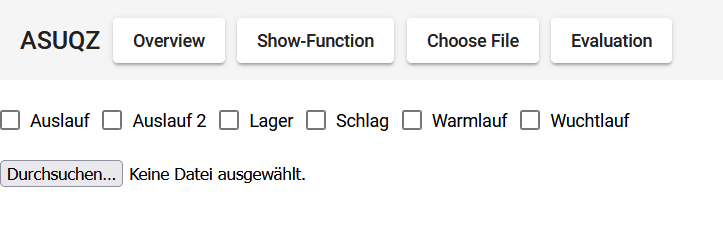
\includegraphics{pics/choosefile.png}
    \caption{Datei auswählen}
    \label{fig:choosefile}
\end{figure}

Wurde eine Datei ausgewählt, wird der Mitarbeiter zur grafischen Auswertung weitergeleitet. Hier kann der Mitarbeiter alle 
verschiedenen Messungen dieser Datei ansehen [\ref{fig:visualization}].
\begin{figure}[h]
    \centering
    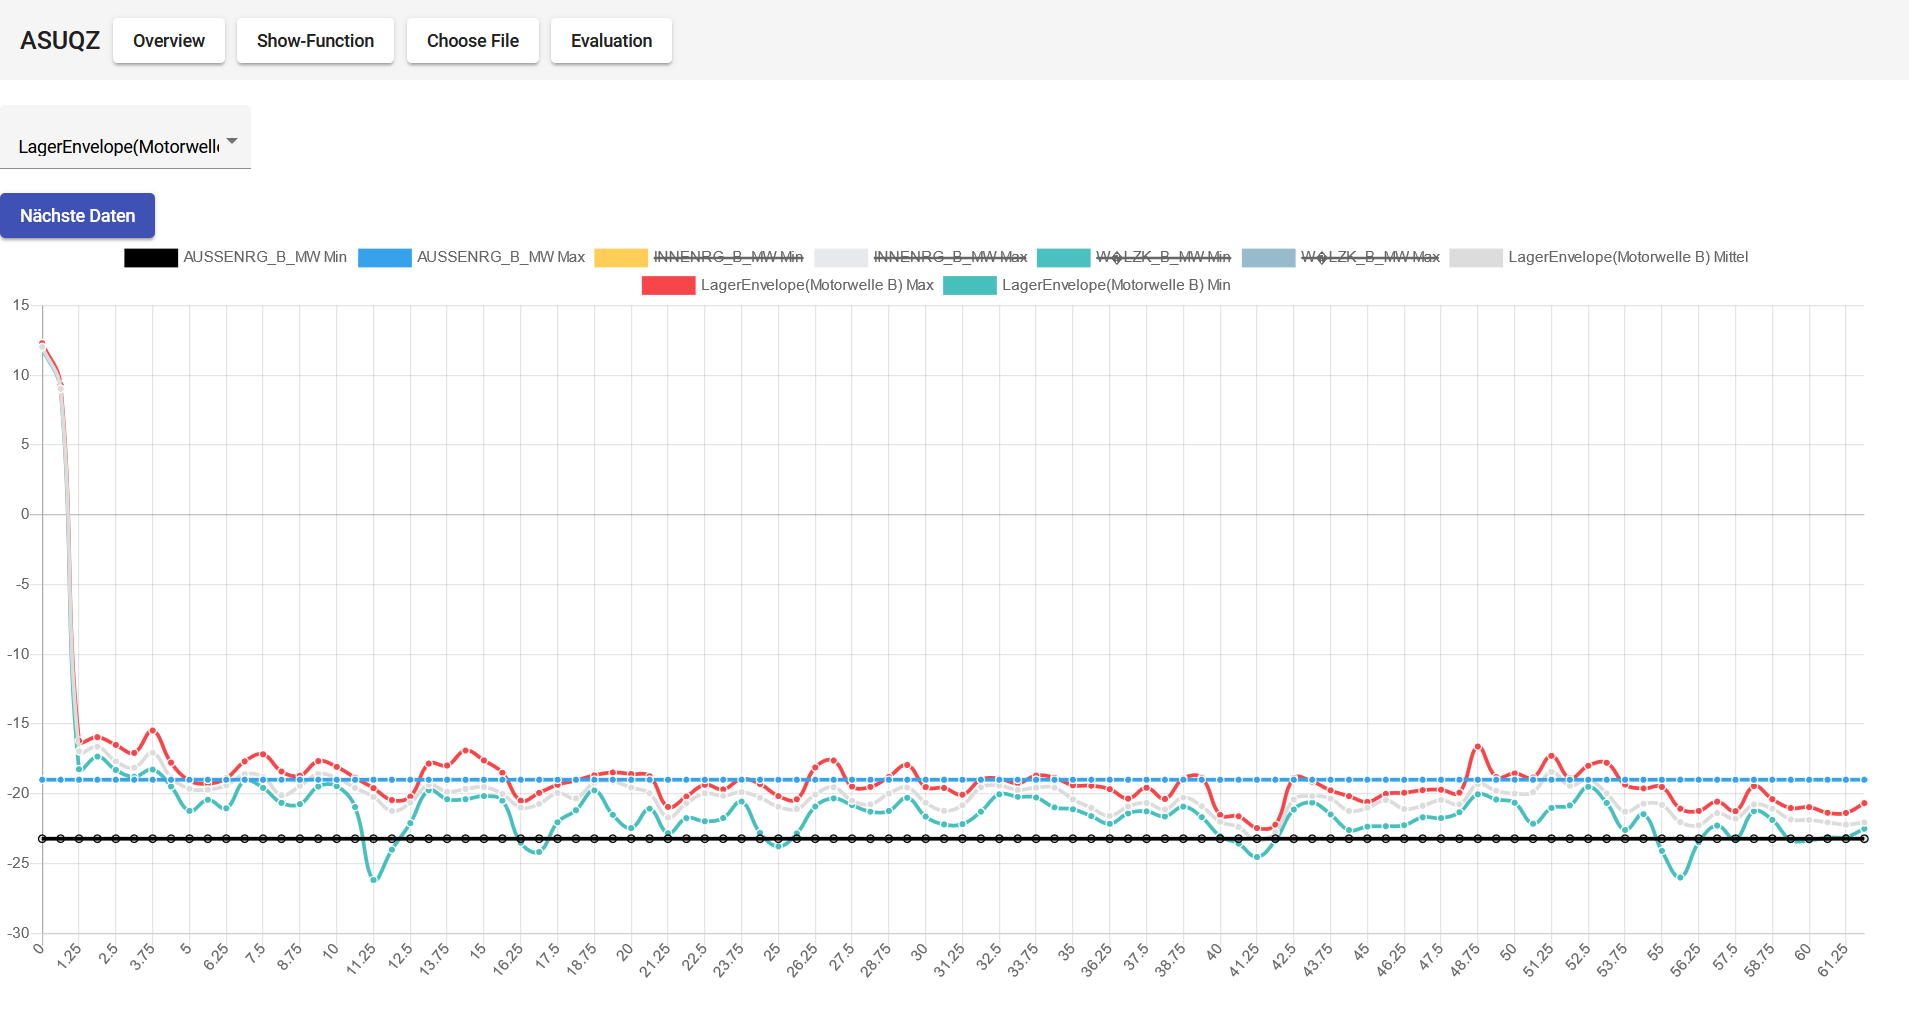
\includegraphics[width=0.80\textwidth]{pics/graph.PNG}
    \caption{Visualisierung}
    \label{fig:visualization}
\end{figure}

Für das Auswerten der Fehler werden die Kriterien in dieser [\ref{fig:evaluation}] Maske ausgewählt.
\begin{figure}[h]
    \centering
    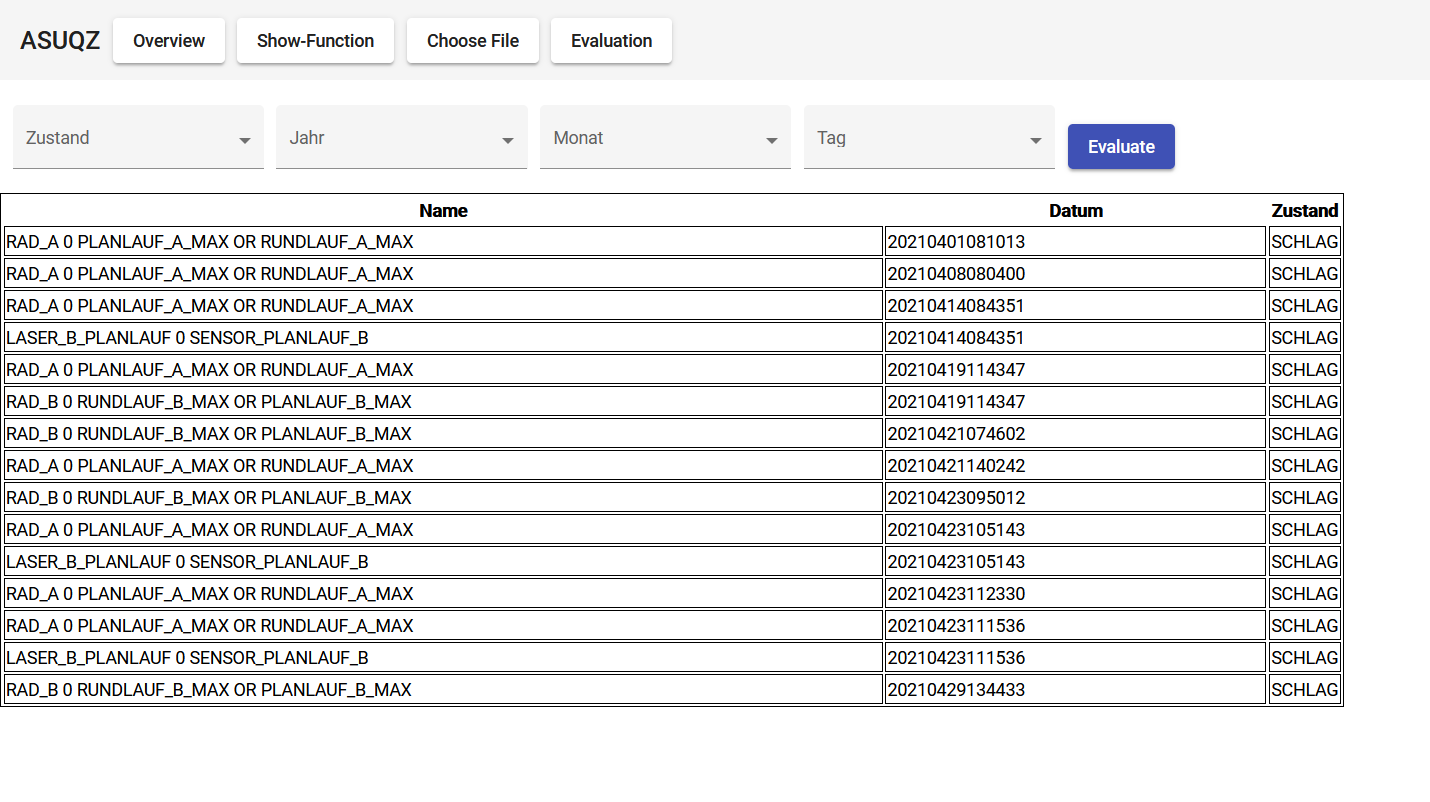
\includegraphics[width=0.80\textwidth]{pics/evaluation.png}
    \caption{Auswertung}
    \label{fig:evaluation}
\end{figure}
